\chapter{Kinematics}

\pagestyle{fancy}
\fancyhf{}
\fancyhead[OC]{\leftmark}
\fancyhead[EC]{\rightmark}
%\renewcommand{\footrulewidth}{1pt}
\cfoot{\thepage}

\section{Key Concepts and Formulae}

\begin{enumerate}
\item Choose the most appropriate frame of reference. Depending on the problem, you may choose an inertial frame, center-of-mass frame, non-inertial frame in which most of the bodies are at rest, or any frame which simplifies the solution.

\item Before starting with the solution, choose the direction of co-ordinate axes and stick with the convention throughout the problem. A negative solution generally signifies that the direction of the quantity is opposite to the assumed direction.

\item Average velocity and acceleration over an interval are 
\begin{align}
\langle\mathbf{v}\rangle &= \frac{\Delta\mathbf{r}}{t} \label{eq1}\\
\langle\mathbf{a}\rangle &= \frac{\Delta\mathbf{v}}{t} \label{eq2}
\end{align}
Bear in mind that these quantities are vectors and should be operated vectorically.

\item Instantaneous velocity and acceleration at a point are
\begin{align}
\mathbf{v} &= \frac{\diff \mathbf{r}}{dt} \label{eq3}\\
\mathbf{a} &= \frac{\diff \mathbf{v}}{dt} \label{eq4}\\
a_x &= v_x\frac{\diff v}{\diff x} \label{eq5}
\end{align}
Remember that a body can be accelerated not only by changing the magnitude of velocity but also by changing the direction of motion, which brings us to

\item It is often convenient to resolve acceleration vector in directions that are tangential and normal to a trajectory.
\begin{align}
a_t &= \frac{\diff |\mathbf{v}|}{\diff t} \label{eq6}\\
a_n &= \frac{v^2}{R} \label{eq7}
\end{align}
Here, $a_t$, the tangential acceleration, can be thought of as the component that measures the change in speed (magnitude of velocity) and $a_n$, the centripeta acceleration, as the component that measures the change in direction of motion or the sharpness of turn. \newline
And, $R$ is the radius of curvature of the trajectory at the given point. For a trajectory $y=f(x)$, $R$ at a point $x$ is given by 
\begin{equation} \label{eq8}
R=\ddfrac{\left(1+\left(\frac{\diff y}{\diff x}\right)^{\!2}\right)^{\!\frac{3}{2}}}{\frac{\Diff2 y}{\diff x^2}}
\end{equation}

\item Distance covered by a body in an interval is given by 
\begin{equation} \label{eq9}
s=\int_{t_1}^{t_2}v_{(t)}\diff t
\end{equation}

\item Angular velocity and angular acceleration of a solid body are
\begin{align}
\bm{\omega} &= \frac{\diff \bm{\theta}}{\diff t} \label{eq10}\\
\bm{\alpha} &= \frac{\diff \bm{\omega}}{\diff t} \label{eq11}
\end{align}
The direction of $\theta$ is assumed to be perpendicular to the plane of rotation and its sense is taken according to the right hand screw rule.

\begin{table}[h]
    \centering
    \begin{tabular}{c  c}
        \begin{minipage}{.48\textwidth}
            \includesvg[width=\linewidth]{figures/kinem/one.svg}
        \end{minipage}
        &
        \begin{minipage}{.48\textwidth}
            \includesvg[width=\linewidth]{figures/kinem/two.svg}
        \end{minipage} \\
        \begin{minipage}{.48\textwidth}
            \begin{itemize}
                \item $\bm{\theta}$ points outward from the plane of the circle.
                \item $\bm{\omega}$ points outward from the plane of the circle.
                \item $\bm{\alpha}$ points inward into the plane of the circle.
            \end{itemize}
        \end{minipage}
        &
        \begin{minipage}{.48\textwidth}
            \begin{itemize}
                \item $\bm{\theta}$ points outward from the plane of the circle.
                \item $\bm{\omega}$ points inward into the plane of the circle.
                \item $\bm{\alpha}$ points inward into the plane of the circle.
            \end{itemize}
        \end{minipage}
    \end{tabular}
\end{table}

\item Linear and rotational quantities are related in the following ways
\begin{align}
\mathbf{v} &= \bm{\omega}\times\mathbf{r} \label{eq12}\\
a_n &= \omega^2R && \text{in the direction oppposite to $\mathbf{r}$} \label{eq13}\\
a_t &= {\omega}R && \text{\begin{tabular}{c}
along the direction of $\mathbf{v}$ if $\mathbf{v}$ is increasing\\
opposite the direction of $\mathbf{v}$ if $\mathbf{v}$ is decreasing
\end{tabular}} \label{eq14}
\end{align}
Here $\mathbf{r}$ is the radius vector of the considered point relative to an arbitrary point on the rotation axis, and $R$ is the distance from the rotation axis.

\end{enumerate}

\begin{note}
The constant-acceleration formulae are
\begin{align}
v_x &= {v_0}_x+a_xt \label{eq15}\\
x&=x_0+{v_0}_x+\frac{1}{2}a_xt^2 \label{eq16}\\
{v_x}^2&={{v_0}_x}^2+2a_x(x-x_0) \label{eq17}\\
x-x_0&=\frac{1}{2}({v_0}_x+v_x)t \label{eq18}
\end{align}
Although these expressions can easily be obtained from \eqref{eq3}, \eqref{eq4} and \eqref{eq5}, it is useful to remember them as they are used often. But, in using them, do not forget that they apply only when the acceleration is constant.
\end{note}

\section{Bridging Problem}

\begin{wrapfigure}{r}{0.3\textwidth}
    \includesvg[width = \linewidth]{figures/kinem/three.svg}
\end{wrapfigure}

You fire a ball with an initial speed $v_0$ at and angle $\phi$ above the surface of an incline which is itself inclined at an angle $\theta$ above horizontal.

\begin{enumerate}[label=\alph*)]
\item Find the distance, measured along the incline, from the launch point to the point where the ball strikes the incline.
\item What angle $\phi$ gives the maximum range measured along the incline?
\end{enumerate}

\textsc{Solution:}

First choose the co-ordinate axes. You could choose x-axis along the incline or along the horizontal. Using the incline is a bit easier, which is why we will choose x-axis along the line the incline the incline and y-axis perpendicular to it.

Our first task is to determine the acceleration along the x and y directions and check whether they are constant.

\begin{wrapfigure}{l}{0.3\textwidth}
    \includesvg[width = \linewidth]{figures/kinem/four.svg}
\end{wrapfigure}

On resolution, we get
\begin{align*}
a_x &= -g\sin\theta \\
a_y &= -g\cos\theta
\end{align*}
both of which are constant. Hence, we may use the constant-acceleration formulae.

Before starting with the solution, it is often convenient to take stock of initial parameters.
\begin{equation*}
{x_0}=0 \quad {y_0}=0 \quad {v_0}_x=v_0\cos\phi \quad {v_0}_y=v_0\sin\phi
\end{equation*}

Now using \eqref{eq16}, we determine $x$ and $y$ as functions of time.

\begin{align}
x_{(t)} &= (v_0\cos\phi)t - \ddfrac{g\sin\theta}{2}t^2 \label{eq19}\\
\text{and} \quad y_{(t)} &= (v_0\sin\phi)t - \ddfrac{g\cos\theta}{2}t^2 \label{eq20}
\end{align}
Next we determine the time $\tau$ it takes for the ball to hit the incline using $y_{(\tau)}=0$.
\begin{equation*}
\tau\biggl(\ddfrac{g\cos\theta}{2}\tau-v_0\sin\phi\biggr)=0
\end{equation*}
Since $\tau=0$ signifies the launch, this solution is trivial.
\begin{equation*}
\therefore \tau= \ddfrac{2v_0\sin\phi}{g\cos\theta}
\end{equation*}
Now we obtain the x distance travelled by the ball in this time by plugging the value of $\tau$ in \eqref{eq19}.
\begin{align}
\text{Range}=R&=x_{(\tau)}=v_0\cos\phi\biggl(\ddfrac{2v_0\sin\phi}{g\cos\theta}\biggr)-\ddfrac{g\sin\theta}{2}\biggl(\ddfrac{2v_0\sin\phi}{g\cos\theta}\biggr)^{\!2}\nonumber\\
\text{On simplification,}\quad R&= \ddfrac{2{v_0}^2\sin\phi\cos(\theta+\phi)}{g\cos^2\theta}\label{eq21}
\end{align}
For part (b) of the problem, we use calculus. In order for $R$ to be maximum, derivative of $R$ with respect to $\phi$ must be zero.
\begin{align}
\ddfrac{\diff}{\diff \phi}\bigl(\sin\phi\cos(\theta+\phi)\bigr)&=0\nonumber\\
\cos(\theta+2\phi)&=0\nonumber\\
\therefore\phi_c&=45\degree-\ddfrac{\theta}{2}\label{eq22}
\end{align}
\textsc{Evaluation:}
\begin{enumerate}

\item Check the dimensions of expression for R \eqref{eq21}.

\item Check the answers in the limiting case of $\theta=0$ and observe if they make sense.
\begin{align*}
R_{(\theta=0)}&=\ddfrac{{v_0}^2\sin2\phi}{g}\\
{\phi_c}_{(\theta=0)}&=45\degree
\end{align*}
Have you seen these results elsewhere?

\end{enumerate}

\section{Level 1 Problems and Solutions}

\begin{enumerate}

\item The velocity of a particle moving in the positive direction of the x-axis varies as $v=\alpha\sqrt{x}$ where $\alpha$ is a positive constant. Assuming that the particle was located at $x=0$ at the moment $t=0$, find
\begin{enumerate}
\item time dependence of velocity and acceleration of the particle.
\item mean velocity of particle averaged over the time that the particle takes to cover the first $s$ meters of the path. \hfill \textsl{Irodov 1.22}
\end{enumerate}

\textsc{Solution:}\\
First find $x$ as a function of time using the given expression and \eqref{eq3}.
\begin{align*}
\ddfrac{\diff x}{\diff t}&=\alpha\sqrt{x}\\
\ddfrac{\diff x}{\sqrt{x}}&=\alpha\diff t
\end{align*}

Since $x=0$ at $t=0$, use these as limits of integration
\begin{align*}
\int_0^xx^{-1/2}\diff x &= \int_0^t \alpha \diff t\\
x_{(t)}&=\ddfrac{\alpha^{2}t^2}{4}\\
\therefore v_{(t)}&= \ddfrac{\diff x}{\diff t}= \ddfrac{\alpha^{2}t}{2}\\
\text{and} \quad a_{(t)} &= \ddfrac{\diff v}{\diff t} = \ddfrac{\alpha^2}{2}
\end{align*}
The following fact will be required to solve part (b)\\
\noindent \fbox{%
\parbox{\textwidth}{%
For a function $y=f(x)$ continuous over the interval $[a,b]$, the average value of y over $[a,b]$ is given by
\begin{equation} \label{eq23}
{y_{av}}_{[a,b]}=\ddfrac{\int_a^b y_{(x)}\diff x}{b-a}
\end{equation}
}%
}
Using \eqref{eq23}, average velocity over a time interval is given by
\begin{equation*}
\langle v \rangle = \ddfrac{\int_{t_1}^{t_2} v_{(t)}\diff t}{t_2-t_1}
\end{equation*}
For this particular problem 
\begin{align*}
t_1=0 \quad \text{and} \quad t_2=\frac{2\sqrt{s}}{\alpha} \qquad \quad \biggl[\because x_{(t)}=\ddfrac{\alpha^{2}t^2}{4}\biggr]
\end{align*}
\begin{equation*}
\langle v \rangle = \ddfrac{\int_0^{t_2} \ddfrac{\alpha^{2}t}{2} \diff t}{t_2} = \ddfrac{\alpha^{2}t_2}{4}
\end{equation*}
Replace the value of $t_2$ to get
\begin{equation*}
\langle v \rangle = \ddfrac{\alpha\sqrt{s}}{2}
\end{equation*}
Check dimensions of all answers.

\item  A point moves along a circle with a velocity $v=at$, where $a=0.50$ \si{m.s^{-1}}. Find the total acceleration of the point at the moment when it covers the $n^{th}$ $(n=0.10)$ fraction of the circle after the beginning of motion. \hfill \textsl{Irodov 1.37}\\

\textsc{Solution:}\\
 Assume circle of radius $R$ and location of point is $\theta=0$ at $t=0$. 
\begin{align*}
\omega_{(t)}&=\ddfrac{v_{(t)}}{R}=\ddfrac{at}{R}\\
\ddfrac{\diff \theta}{\diff t}&=\ddfrac{at}{R}
\end{align*}
When the circle covers $n^{th}$ fraction of the circle, $\theta=2\pi n$ 
\begin{align*}
\int_0^{2\pi n} R \diff \theta &= \int_0^\tau at \diff t\\
\therefore \tau &= \sqrt{\ddfrac{4\pi nR}{a}}
\end{align*}
For a particle in circular motion, it is easier to think of its acceleration in terms of its tangential and normal components.Using \eqref{eq6} and \eqref{eq7}, we get
\begin{align*}
a_t &= \frac{\diff}{\diff t}(at) = a\\
a_n &= \omega^2 R = \frac{a^2 t^2}{R}\\
\text{For $t=\tau$}, \\
a_n&= 4\pi an\\
\text{So, the total acceleration at $t=\tau$ is}\\
a_{tot} &= \sqrt{{a_t}^2+{a_n}^2}\\
a_{tot} &= a\sqrt{1+{(4\pi n)}^2}\\
\text{put $a=0.50$ \si{m.s^{-2}} and $n=0.10$},\\
a_{tot}&= 0.81 \quad \si{m.s^{-2}}
\end{align*}
Note the use of significant figures.

\item An airplane pilot wishes to fly due west. A wind of 80.0 \si{km/h} is blowing toward the south. 
\begin{enumerate}
\item If the airspeed of the plane in still air is 320.0 km/h, in which direction should the pilot head?
\item What is the speed of plane over the ground? 
\end{enumerate}
Draw a vector diagram. \hfill \textsl{UP 3.38}

\textsc{Solution:}\\
$\mathbf{v}_{W/G}$ = velocity of wind w.r.t. ground\\
$\mathbf{v}_{P/G}$ = velocity of plane w.r.t. ground\\
$\mathbf{v}_{P/W}$ = velocity of plane w.r.t. wind (or velocity in still air)\\
The vector diagram of the situation described above is shown below\\

\begin{figure}[hbt]
    \centering
    \includesvg{figures/kinem/five.svg}
\end{figure}

Relative velocities can be written in vectorical form as shown below.
\begin{align*}
    \mathbf{v}_{P/W}&=\mathbf{v}_{P/G}+\mathbf{v}_{G/W}\\
    \mathbf{v}_{P/W}&=\mathbf{v}_{P/G}+(-\mathbf{v}_{W/G})
\end{align*}

So the direction of $\mathbf{v}_{P/W}$ or the direction pilot should head for is shown in the vector diagram below\\

\begin{figure}[hbt]
    \centering
    \includesvg{figures/kinem/six.svg}
\end{figure}

Using Pythagorean theorem in the right triangle
\begin{align*}
{v_{P/W}}^2&={v_{P/G}}^2+{v_{W/G}}^2\\
v_{P/G}&=\sqrt{{v_{P/W}}^2-{v_{W/G}}^2}\\
\text{And} \quad \sin\theta &= \ddfrac{v_{W/G}}{v_{P/W}}\\
\theta &= \sin^{-1}\biggl(\ddfrac{v_{W/G}}{v_{P/W}}\biggr)
\end{align*}
Use $v_{W/G}$=80.0 km/h and $v_{P/W}$=320.0 km/h,
\begin{equation*}
v_{P/G}=309.8 \si{km/h} \quad \text{and} \quad \theta=14.5\degree
\end{equation*}
The pilot should head 14.5\degree  north of west and the speed of plane over the ground is 309.8 km/h.

\item A particle moves along a parabola $y=ax^2$ with velocity $\mathbf{v}$ whose modulus is constant. Find the acceleration of the particle at the point $x=0$. \hfill \textsl{NePhO 2018}

\textsc{Solution:}\\
Think of the particle's acceleration in terms of its tangential and normal components.
\begin{align*}
a_t&=\ddfrac{\diff}{\diff t}|\mathbf{v}|\\
\text{But $|\mathbf{v}|$ is constant, so} \quad a_t&=0\\
a_n&=\ddfrac{v^2}{R}
\end{align*}
Here, $R$ is radius of curvature of the parabola $y=ax^2$ at $x=0$. For $R$, use \eqref{eq8}.
\begin{align*}
R&=\ddfrac{\left(1+\left(\frac{\diff y}{\diff x}\right)^{\!2}\right)^{\!\frac{3}{2}}}{\frac{\Diff2 y}{\diff x^2}}\\
&=\ddfrac{(1+2ax)^{\frac{3}{2}}}{2a}\\
&=\frac{1}{2a}\\
\therefore a_n&= 2av^2\\
\text{Finally}, \quad a_{tot}&=a_n=2av^2
\end{align*}
Check dimensions of the final answer.

%\item What work should a man do to walk up a subway escalator moving down? The height of the escalator is 'H', its speed is constant and equal to 'V', and it is inclined at an angle $\alpha$ . 
%
%\textsc{Solution:}\\
%Hint: Work done = F d. \end{align*} 
%what is the total distance covered by man?[keep in mind that the escalator is also moving]
%Ans: W = mgsin\alpha(\frac{h}{sin\alpha} + Vt)

\end{enumerate}

\section{Level 2 Problems and Solutions}

\begin{enumerate}

\item A ball is thrown at speed $v$ from zero height on level ground. Let $\theta_0$ be the angle at which the ball should be thrown so that the length of the trajectory is maximum. Show that $\theta_0$ satisfies
\begin{align*}
\sin\theta_0\ln\biggl(\ddfrac{1+\sin\theta_0}{\cos\theta_0}\biggr)=1  &&\textsl{Morin 3.19}
\end{align*}
\textsc{Solution:}\\
First let's obtain the equation of trajectory of the ball.
\begin{align*}
x_{(t)}&=(v\cos\theta)t\\
y_{(t)}&=(v\sin\theta)t-\frac{gt^2}{2}
\end{align*}
Eliminating $t$ from these equations, we get
\begin{equation*}
y_{(x)}=(\tan\theta)x-\frac{g}{2v^2\cos^2\theta}x^2
\end{equation*}
For length of the trajectory, 
\begin{equation} \label{eq24}
L=\mathlarger{ \int_0^R} \sqrt{1+\biggl(\ddfrac{\diff y}{\diff x} \biggr)^{\!2}} \diff x
\end{equation}
Here $R=\ddfrac{v^2\sin2\theta}{g}$ is the range of the ball. \eqref{eq24} is easily understood if you consider infinitesimal length $\diff L = \sqrt{(\diff x)^2+(\diff y)^2}$.
\begin{align}
L&=\int_0^{\frac{v^2\sin2\theta}{g}} \sqrt{1+\biggl( \tan\theta - \ddfrac{g}{v^2\cos^2\theta}x\biggr)^{\!2}} \diff x \nonumber
\end{align}
Substitute $\tan\theta-\ddfrac{g}{v^2\cos^2\theta}x=u$,
\begin{align}
&= \ddfrac{v^2\cos^2\theta}{g}\int_{-\tan\theta}^{\tan\theta} \sqrt{1+u^2} \diff u \nonumber
\end{align}
Since the integrand is an even function,
\begin{align}
&= \ddfrac{2v^2\cos^2\theta}{g}\int_0^{\tan\theta} \sqrt{1+u^2} \diff u \nonumber\\
&= \ddfrac{2v^2\cos^2\theta}{g}.\ddfrac{1}{2} \bigl(u\sqrt{1+u^2}+\ln(u+\sqrt{1+u^2}) \bigr)\biggr|_0^{\tan\theta} \nonumber\\
\therefore L &= \ddfrac{v^2}{g}\biggl(\sin\theta + \cos^2\theta\ln\biggl(\ddfrac{1+\sin\theta}{\cos\theta} \biggr) \biggr) \label{eq25}
\end{align}
In order for $L$ to be maximum, the derivative of $L$ with respect to $\theta$ should be zero.
\begin{equation*}
\cos\theta - 2\cos\theta\sin\theta\ln\biggl(\ddfrac{1+\sin\theta}{\cos\theta} \biggr) + \cos^2\theta \biggl(\ddfrac{\cos\theta}{1+\sin\theta} \biggr)\ddfrac{\cos^2\theta+(1+\sin\theta)\sin\theta}{\cos^2\theta}=0
\end{equation*}
On simplification, this reduces to 
\begin{equation*}
\sin\theta\ln\biggl(\ddfrac{1+\sin\theta}{\cos\theta} \biggr)=1
\end{equation*}
On solving this equation, we get $\theta_0$ for which length of trajectory is maximum.
\begin{note}
\begin{enumerate}
\item Check the expression for $L$ \eqref{eq25} in the limiting cases of $\theta=0\degree$ and $\theta=90\degree$ and observe if the results make sense.
\item In some IPhO problems, you will be asked to solve equations like these numerically. We strongly recommend you learn at least one numerical method and as an exercise, we will leave it to you to verify that the solution for $\theta$ is $\theta_0\approx56.5\degree$.
\end{enumerate}
\end{note}

\item A solid body rotates with a constant angular velocity $\omega_0=0.5$ rad/s about a horizontal axis AB. At the moment $t=0$, the axis AB starts turning about the vertical with a constant angular acceleration $\beta_0=0.10$ \si{rad/s^2}. Find the angular velocity and angular acceleration of the body after $t=3.5$ s. \hfill \textsl{Irodov 1.58} 

\textsc{Solution:}\\
Consider unit vectors $\mathbf{i}$ in the direction of axis AB, $\mathbf{k}$ perpendicular to AB in the plane of rotation and $\mathbf{j}$ perpendicular to the plane of rotation of AB as shown.

\begin{figure}[hbt]
    \centering
    \includesvg{figures/kinem/seven.svg}
\end{figure}

\begin{align*}
\bm{\omega_P} &= \omega_0\mathbf{i} + \beta_0t\mathbf{j}\\
|\bm{\omega_P}|&= \sqrt{{\omega_0}^2+{\beta_0t}^2}
\end{align*}
For $\bm{\alpha_P}$,
\begin{align*}
\bm{\alpha_P}&=\ddfrac{\diff \bm{\omega_P}}{\diff t}=\frac{\diff}{\diff t}(\omega_0\mathbf{i} + \beta_0t\mathbf{j})
\end{align*}
Vector differentiation will be used to obtain the solution. Note that vector differentiation is equivalent to using product rule of differentiation on a vector assuming it to be a product of a scalar and a vector
\begin{align*}
\bm{\alpha_P}&=\omega_0\frac{\diff \mathbf{i}}{\diff t} + \mathbf{i}\frac{\diff \omega_0}{\diff t} + \beta_0t\frac{\diff \mathbf{j}}{\diff t} + \mathbf{j}\frac{\diff (\beta_0t)}{\diff t}\\
\text{Here}, \quad \frac{\diff \omega_0}{\diff t} &= 0 \quad \frac{\diff \mathbf{j}}{\diff t}=0 \quad \frac{\diff \mathbf{i}}{\diff t} = \beta_0t \mathbf{k}\\
\therefore \bm{\alpha_P}&= \omega_0\beta_0t\mathbf{k}+\beta_0\mathbf{j}\\
|\bm{\alpha_P}|&= \beta_0\sqrt{1+{\omega_0}^2t^2}
\end{align*}
Plug $\omega_0=0.50$ rad/s, $\beta_0=0.10$ \si{rad/s^2} and $t=3.50$ s.
\begin{align*}
\omega_P=0.61 \si{ rad/s} \quad \text{and} \quad \alpha_P=0.20 \si{ rad/s^2}
\end{align*}

\begin{minipage}{0.6\textwidth}
    The direction of $\frac{\diff \bm{i}}{\diff t}$ is $\bm{k}$ for the same reason that direction of centripetal acceleration is perpendicular to velocity in uniform circular motion. Consider the figure where $\bm{i_1}$ is the initial direction of axis AB and $\bm{i_2}$ is the direction after time $\Delta t$. The direction of $\Delta \bm{i}$ is as shown. In the limit of $\Delta t \to 0$, $\bm{i_2} \to \bm{i_1}$ and hence the direction of $\diff \bm{i}$ is perpendicular to $\bm{i}$ and along $\bm{k}$.
\end{minipage} \hspace{0.05\textwidth}
\begin{minipage}{0.25\textwidth}
    \includesvg[width = \linewidth]{figures/kinem/eight.svg}
\end{minipage}

\end{enumerate}

\section{IPhO Problems}

A ball, thrown with an initial speed $v_0$, moves in a homogeneous gravitational field in the x-z plane, where the x-axis is horizontal, and the z-axis is vertical and antiparallel to the free fall acceleration $g$ . Neglect the effect of air drag.
\begin{enumerate} [label=\roman*)]
\item By adjusting the launching angle for a ball thrown with a fixed initial speed $v_0$ from the origin, targets can be
hit within the region given by
\begin{equation} \label{eq26}
z \leq z_0 - kx^2
\end{equation}
You can use this fact without proving it. Find the constants $z_0$ and $k$.
\item The launching point can now be freely selected on the ground level $z = 0$, and the launching angle can be adjusted as needed. The aim is to hit the topmost point of a spherical building of radius $R$ (see fig.) with the
minimal initial speed $v_0$. Bouncing off the roof prior to hitting the target is not allowed. Sketch qualitatively the shape of the optimal trajectory of the ball. 
\item What is the minimal launching speed $v_{min}$ needed
to hit the topmost point of a spherical building of radius $R$? \hfill \textsl{IPhO 2012 Estonia}

\end{enumerate}

\textsc{Solution:}

\begin{enumerate} [label=\roman*]
\begin{minipage}{0.6\textwidth}
    \item The maximum heght $z_0$ is achieved when the ball is thrown vertically upwards.
\begin{equation} \label{eq27}
z_0=\ddfrac{{v_0}^2}{2g}
\end{equation}
The maximum horizontal distance is achieved when the ball is thrown at an angle of 45\degree and the distance covered in that case is $\ddfrac{{v_0}^2}{g}$. But using \eqref{eq26}, the maximum horizontal distance achievable is $\sqrt{\ddfrac{z_0}{k}}$.
\end{minipage}
\begin{minipage}{0.3\textwidth}
    \includesvg[width=\linewidth]{figures/kinem/nine.svg}
\end{minipage}

\begin{align}
\sqrt{\ddfrac{z_0}{k}}&=\ddfrac{{v_0}^2}{g} \nonumber\\
k&= \frac{g}{2{v_0}^2} \label{eq28}
\end{align}
\item In kinematics, it is sometimes easier to analyze a process by reversing it. In this case, we can ask ourselves: What is the trajectory of the ball thrown from the roof of the building with minimum initial speed such that it does not hit the building on its way down?\\
With purely qualitative reasoning, we arrive at the conclusion that the ball must touch the building on its way down. For example, say a ball is thrown at an angle from the roof and its trajectory does not touch the building. Then we can argue that the ball can be thrown at the same angle by lowering its speed continually until the trajectory just touches the roof at some point. The speed can't be lowered any further as the ball would then hit the roof.

\begin{minipage}{0.6\textwidth}
    Now assume the ball is thrown horizontally from the roof. We can increase the throwing angle slightly upward while keeping the same speed. This trajectory would not touch the building at any point. Now we can use the same argument to conclude that the speed can still be lowered until the trajectory touches the building.\\
    So the optimal trajectory must touch the building at some point as shown.
\end{minipage}
\begin{minipage}{0.3\textwidth}
    \includesvg[width=\linewidth]{figures/kinem/ten.svg}
\end{minipage}

\item Before getting into the solution, it is essential to distinguish between targetable region and trajectory. Trajectory is the actual path the ball travels through when thrown from a point with a particular speed and at a particular angle. Targetable region, on the other hand, includes all possible trajectories the ball can trace when thrown from a point with a particular speed at different angles. We established in the solution to ii) that the optimal trajectory must touch the building. By similar analysis, we can also show that boundary of targetable region for minimum speed must also touch the building. If it were to not touch the building, it would be possible to throw the ball along any one trajectory that does not touch the building. Again it would be possible to further lower the speed hence we can conclude that the initial speed could not have been the minimum speed. So, the boundary of targetable region for minimum speed must touch the building. The equation of this boundary when a ball is thrown from origin with a speed $v_0$ is given below, using \eqref{eq26}, \eqref{eq27} and \eqref{eq28}:
\begin{equation*}
z=\ddfrac{{v_0}^2}{2g}-\ddfrac{gx^2}{2{v_0}^2}
\end{equation*}
Now take origin at the top of spherical building, the equation of the spherical building in x-z plane is
\begin{align*}
x^2+(z+R)^2&=R^2\\
x^2+z^2+2zR&=0
\end{align*}
Eliminating $z$ from these equations, we get the following equation, biquadratic in x.
\begin{equation} \label{eq29}
\ddfrac{g^2}{4{v_0}^4}x^4+\biggl(\ddfrac{1}{2}-\ddfrac{gR}{{v_0}^2}\biggr)x^2+\biggl(\ddfrac{{v_0}^4}{4g^2}+\ddfrac{{v_0}^2R}{g}\biggr)=0
\end{equation}
Let's pause for a moment to understand the implications of \eqref{eq29}. If the value of $v_0$ is less than the minimum speed, it will have four solutions because the boundary of targetable region and circle will intersect at four points. (Do not forget that the ball can be thrown in either direction from the top.) If the value of $v_0$ is too large, they will not intersect at all and \eqref{eq29} will have no real solutions. If $v_0$ is the minimum speed, then the boundary of targetable region touches the circle at two points and hence two real solutions are obtained. \\
Recall from your algebra classes that this transition between distinct real roots and imaginary roots takes place when the discriminant equals zero.
\begin{equation*}
\biggl(\ddfrac{1}{2}-\ddfrac{gR}{{v_0}^2} \biggr)^{\!2} - 4.\ddfrac{g}{4{v_0}^4}.\biggl(\ddfrac{{v_0}^4}{4g^2}+\ddfrac{{v_0}^2R}{g}\biggr)=0
\end{equation*}
On solving for $v_0$, we get
\begin{equation*}
v_0=\sqrt{\ddfrac{gR}{2}}
\end{equation*}
Now would be a great time to blunder by stopping here and recording this as your final answer. Remember that we have been considering the reverse process of throwing the ball off the roof while the problem is concerned with throwing the ball off the ground. So you have to find the speed of the ball when it reaches the ground and that is the required $v_{min}$.
\begin{align}
v_{min}&=\sqrt{{v_0}^2+2g(2R)}\nonumber\\
\therefore v_{min}&= 3\sqrt{\ddfrac{gR}{2}} \label{eq30}
\end{align}

\begin{note}
\begin{enumerate}
\item The reverse process can be considered only if the principle of conservation of energy is valid. From an energy standpoint, it is the same thing to throw the ball from the roof as it is from the ground.

\item At this point, you might be wondering why we used the formula of discriminant of quadratic equation in a biquadratic equation. Note that biquadratic equation is, in essence, a quadratic equation if you replace $x^2$ by $y$.
\end{enumerate}
\end{note}

\end{enumerate}

\section{Supplementary Problems}

\begin{enumerate}

\item Three points are located at the vertices of an equilateral triangle whose side equals $a$. They all start moving simultaneously with velocuty $v$ constant in modulus, with the first heading continually for the second, the second for the third, and the third for the first. How soon will the points converge? \hfill \textsl{Irodov 1.12}

\item A balloon starts rising from the surface of the Earth. the ascension rate is constant and equal to $v_0$. Due to the wind the balloon gathers the horizontal velocity component $v_x=ay$, where $a$ ia a constant and $y$ is the height of ascent. Find how the following quantities depend on the height of ascent:
\begin{enumerate}
\item the horizontal drift of the balloon $x(y)$;
\item the total, tangential, and normal accelerations of the balloon. \hfill \textsl{Irodov 1.34}
\end{enumerate}

\item A cylinder rolls without slipping over a horizontal plane The radius of the cylinder is equal to $r$. Find the curvature radii of trajectories traced out by points A and B (see fig.). \hfill \textsl{Irodov 1.54}

\item A car slides without friction down a ramp described by a height function h(x)
which is smooth and monotonically decreasing as x increases from 0
to L. The ramp is followed by a loop of radius R. Gravitational acceleration 
is a constant g in the negative direction.\\ 
\begin{figure}[htp]
    \centering
    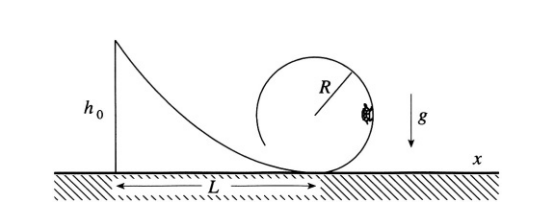
\includegraphics{figures/kinem/kinem2.PNG}
    \label{fig:my_label}
\end{figure}\\
If the velocity is zero when x = 0, what is the minimum height h$_0$ = h(0)
such that the car goes around the loop, never leaving the track?
\hfill \textsl{(Stony Brook)}\\
\big[\textbf{Ans: }h$_0$ = $\dfrac{5}{2}$R\big]
\item A spacecraft in flight explodes into three equal portions. A portion continues along the original line of 
flight. The other two shoot out in directions forming an angle of 60 ° with the original path. The energy 
released in the explosion is twice larger than the kinetic energy possessed by the probe precisely at the time of the 
explosion. Determine the kinetic energy of each fragment immediately after the explosion. \\\hfill \textsl{(CoPhO)}

\item A mass is attached to the end of a string. The mass moves on a frictionless table, and the string passes through a hole in the table (see Figure
P.1.9), under which someone is pulling on the string to make it taut at all
times. Initially, the mass moves in a circle, with kinetic energy The
string is then slowly pulled, until the radius of the circle is halved. How much work was done?\hfill \textsl{(MIT)}
\begin{figure}[htp]
    \centering
    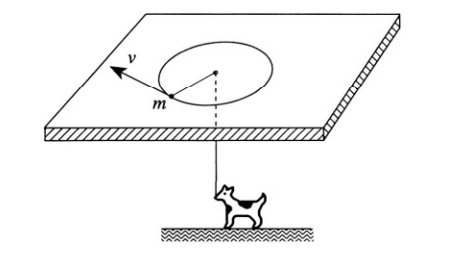
\includegraphics{figures/kinem/kinem3.PNG}
    \label{fig:my_label}
\end{figure}
\textbf{Ans:}$\dfrac{3m^2v^2R^2}{2mR^2} = 3E_0$
\item A cylinder of mass M and radius R is placed on an inclined plane with angle of inclination $\theta$. The 
inclined plane has acceleration $a_o$ with respect to an inertial frame as shown in the figure.

\item A wheel with radius R is situated at height R from
the ground and is rotating at angular velocity $\Omega$. At some point A, a drop of water separates from the wheel and reaches the ground at point B situated directly below the wheel’s axle (see the figure). Find the falling time of the drop and the location of point A (i.e. angle $\alpha$).

\end{enumerate}



